\section{Formal Analysis using Alloy}
\subsection{What we want to model?}

Using Alloy we want to show possible scenarios in which the system can be and we also want to test its correctness.
In particular we are interested in show the following things:
\begin{itemize}
    \item User send Reports
    \item Authority access the Report by the ReportManager
    \item Authority can generate TrafficTickets
    \item TrafficTicket refer to a Report
    \item Report is about a violation made in a Location of a Municipality
    \item Authority can generate TrafficTickets only for violations made in the same Municipality they belong to.
    \item SuggestionsManager take data form ReportManager and form Municipality to cross them and create suggestions. Both User and Authority can access SuggestiosManager to read suggestions about possible improvements
\end{itemize}

\vspace{20px}

\subsection{Alloy Model}
\vspace{10px}
\begin{minted}{alloy}

open util/integer

-- MODEL SIGNATURES --

sig Report{
    reportID: one Int,
	location: one Location
}

abstract sig Guest {
	sm: one SuggestionsManager
}

sig User extends Guest{
	userID: one Int,
	reports: set Report
}

sig Authority extends Guest{
	authID: one Int,
	rm: one ReportManager,
	trafficTickets: set TrafficTicket,
	municipality: one Municipality
}

one sig ReportManager{
	reports: set Report
}

sig TrafficTicket{
	ticketID: one Int,
	report: one Report,
	municipality: one Municipality
}

sig Location{
	municipality: one Municipality
}

sig Municipality{}

one sig SuggestionsManager{
	rm: one ReportManager,
	municipalities: set Municipality
}


-- FACTS THAT DEFINE THE MODEL --

-- define unique key for Authority --
fact uniqueAuthorityID{
	no disj a1, a2: Authority | a1.authID = a2.authID			
}

-- define unique key for Report --
fact uniqueReportID{
	no disj r1, r2: Report | r1.reportID = r2.reportID			
}


-- define unique key for User --
fact uniqueUserID{
	no disj u1, u2: User | u1.userID = u2.userID			
}

-- define unique key for TrafficTicket --
fact uniqueTrafficTicketID{
	no disj tt1, tt2: TrafficTicket | tt1.ticketID = tt2.ticketID			
}

fact ownReport{
	-- all report are generated by only one user --
	all r: Report |
		no disj u1,  u2: User |
			r in u1.reports and r in u2.reports

	-- all report are generated by someone --
	all r: Report |
		one u: User |
			r in u.reports
}

fact ownTrafficTicket{
	-- all traffic tickets are generated by only one authority --
	all tt: TrafficTicket |
		no disj a1,  a2: Authority |
			tt in a1.trafficTickets and tt in a2.trafficTickets

	-- all traffic tickets are generated by someone --
	all tt: TrafficTicket |
		one a: Authority |
			tt in a.trafficTickets
}

--  Report can't stay into different TrafficTicket --
fact trafficTicketReport{
	all r: Report |
		no disj tt1, tt2: TrafficTicket | r = tt1.report and
		                                  r = tt2.report
}




-- all the Reports are managed by the ReportManager
fact manageOnce{
	all r: Report | 
		one rm: ReportManager | 
			r in rm.reports
}

/* Authority can generate TrafficTicket only for violations made
     into the same municipality in which it is registered */
fact checkAuthorityZone{
	all tt: TrafficTicket |
		one r: Report |
			r = tt.report and tt.municipality =
				        r.location.municipality

	all tt: TrafficTicket |
		one a: Authority |
			tt in a.trafficTickets and a.municipality =
			                            tt.municipality
}

-- SuggentionsManager must see all the Municipalities in order to collect data --
fact SugManagerSeeAllMunicipalities {
	all m: Municipality |
		one sm: SuggestionsManager |
			m in sm.municipalities
}

\end{minted}

\newpage

\subsection{Alloy generated Worlds}
    \vspace{10px}
    \begin{itemize}
        \item \textit{\textbf{Simple case}}: Here we can see the case in which a User has sent a Report, an Authority has verified it and a TrafficTicket has been generated.\\\\
        To obtain this world representation the line of Alloy code about the SuggestionsManager are not executed, while the code for the execution is the following:
        
\begin{minted}{alloy}
    pred show{
        #User = 1
        #Authority = 1
        #TrafficTicket = 1
        #Report = 1
    }
    
    run show for 3
\end{minted}
        
        \begin{figure}[h]
            \centering
            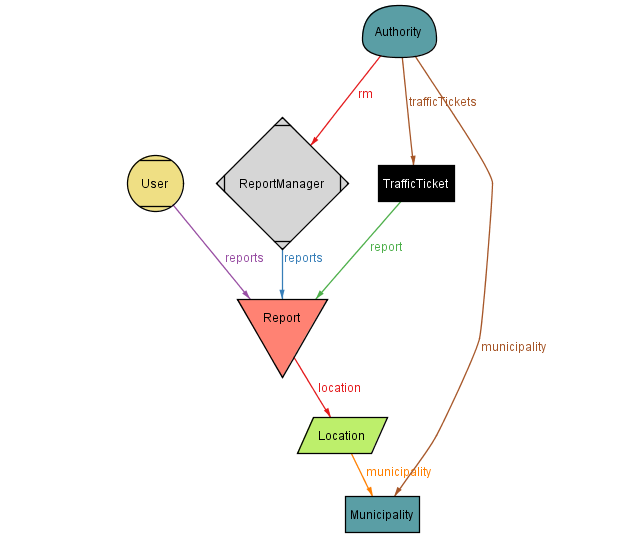
\includegraphics[scale=0.5]{Images/alloy_simple.png}
        \end{figure}
        
        \vspace{40px}
        
        
        \item \textit{\textbf{More Entities}}: In this case we can see the same things as before but in a more complex situation because there are more Entities. Here we can also notice that the Authority can generate a TrafficTicket only to Reports made in the Municipality he belongs to.
        There also is a Report (Report0) in which there is no association we a TrafficTicket. This means that it can be not checked yet or it is verified but the TrafficTicket will be generated after.\\\\
        Here again the code about SuggestionsManager is not executed and the execution code is:
        
\begin{minted}{alloy}
    pred show{
        #User = 3
        #Authority = 2
        #TrafficTicket = 2
    }
    
    run show for 3
\end{minted}

\vspace{1cm}
        
        \begin{figure}[h]
            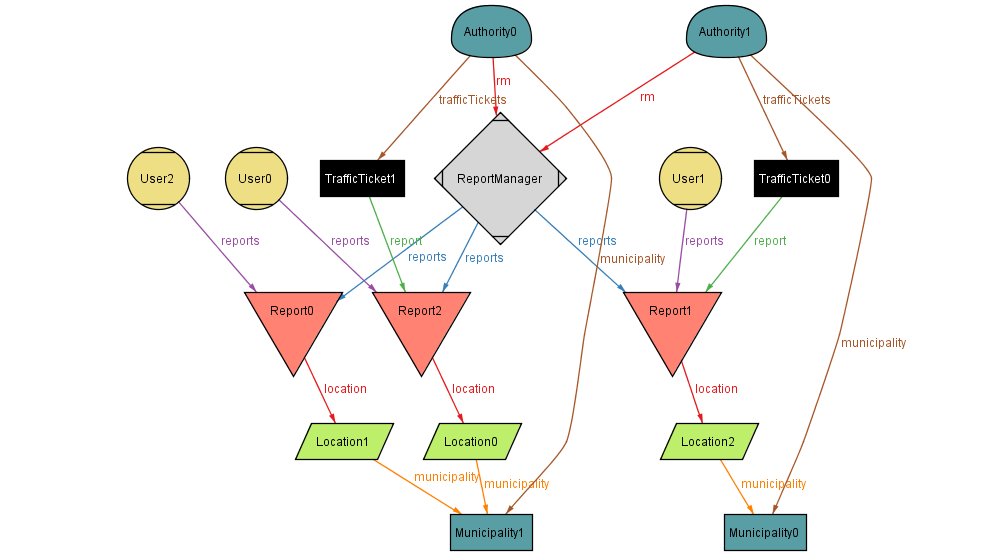
\includegraphics[scale=0.4]{Images/alloy_complex.png}
        \end{figure}
        
\newpage
        \vspace{30px}
        
        
        \item\textit{\textbf{Allows Suggestions}}: This World represent the complete scenario.
        There is what we have discuss before and the insertion of a SuggestionsManager which collect data from Municipalities and Reports (via ReportManager) and cross them to create Suggestion on how to improve urban mobility.
        Both Users and Authorities can access it to read them. Even if a User never send a Report can look at the Suggestions.\\\\
        In this last case the code about SuggestionsManager is executed and to get the model representation the code is:
        
\begin{minted}{alloy}
    pred show{
        #User = 3
        #Authority = 2
        #TrafficTicket = 2
    }
    
    run show for 3
\end{minted}

\vspace{1cm}
        
        \begin{figure}[h]
            \centering
            \advance\leftskip-2cm
            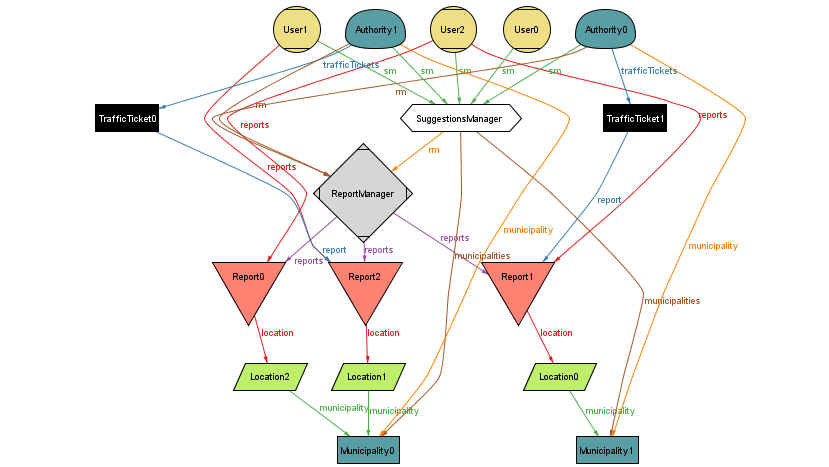
\includegraphics[scale=0.6]{Images/alloy_suggestions.png}
        \end{figure}
        
        \vspace{30px}
    
    
    \end{itemize}